\documentclass{article}
\usepackage[margin=1.0in]{geometry}
\usepackage{amsmath, amssymb, mathrsfs}
\usepackage[english]{babel}
\usepackage{graphicx}
\usepackage{enumerate}
\usepackage{tikz}
\usetikzlibrary{shapes,backgrounds}

\title{Numerical Computing HW 3}
\author{Greg Stewart}
\date{\today}

\begin{document}

\maketitle

\section*{5.2}

\begin{table}[h!]
  \centering
  \begin{tabular} {c | c c c c }
    $x$ & -1 & 0 & 1 & 2 \\ 
    \hline  
    $y$ & 0 & 1 & 1 & 0 \\
  \end{tabular}
\end{table}


\begin{enumerate}[(a)]
  \item \textit{Find the piecewise linear interpolation function $g(x)$ that fits these data.}

    We need the interpolation function
    \begin{align*}
      g(x) &= y_1G_1(x) + y_2G_2(x) + y_3G_3(x) + y_4G_4(x)\\
      &= 0 + G_2(x) + G_3(x) + 0
    \end{align*}
    To do this we need the "hat" function
    \[
      G_i(x) =
      \begin{cases}
        \frac{x-x_{i-1}}{x_i-x_{i-1}} &\text{ if } x_{i-1} \leq x \leq x_i \\
        \frac{x-x_{i+1}}{x_i - x_{i+1}} &\text{ if } x_i \leq x \leq x_{i+1} \\
        0 &\text{ otherwise } \\
      \end{cases}
    \]
    Obviously, we only need $G_2$ and $G_3$:
    \[
      G_2(x) =
      \begin{cases}
        \frac{x+1}{0 + 1} = x + 1&\text{ if } x_{i-1} \leq x \leq x_i \\
        \frac{x-1}{0 - 1} = 1 - x&\text{ if } x_i \leq x \leq x_{i+1} \\
        0 &\text{ otherwise } \\
      \end{cases}
    \]
    \[
      G_3(x) =
      \begin{cases}
        \frac{x-0}{1 - 0} = x &\text{ if } x_{i-1} \leq x \leq x_i \\
        \frac{x-2}{1 - 2} = 2 - x&\text{ if } x_i \leq x \leq x_{i+1} \\
        0 &\text{ otherwise } \\
      \end{cases}
    \]
    So in the end we have

    \[
      g(x) = G_2(x) + G_3(x)
    \]

        
  \item \textit{Find the global interpolation polynomial $p_3(x)$ that fits these data.}

    To find this interpolation we just need to solve a relatively simple matrix equation guaranteeing all data are plotted by the interpolation, which is

  $$
  \begin{pmatrix}
    1 & -1 & 1 & -1 \\ 1 & 0 & 0 & 0 \\ 1 & 1 & 1 & 1 \\ 1 & 2 & 4 & 8 
  \end{pmatrix}
    \begin{pmatrix}
      a_0 \\ a_1 \\ a_2 \\ a_3
    \end{pmatrix}
    =
    \begin{pmatrix}
      0 \\ 1 \\ 1 \\ 0
    \end{pmatrix}
  $$
    Solving this we for $a_i$, we get $a_0 = 1$, $a_1 = \frac{1}{2}$, $a_2 = -\frac{1}{2}$, and $a_3 = 0$, so we can write the polynomial interpolation function

    $$p_3(x) = 1 + \frac{1}{2}x - \frac{1}{2}x^2$$

\end{enumerate}

\section*{5.8(b) \normalsize For the following functions, determine the step size $h$ that will guarantee that the error is less than $10^{-6}$ using piecewise linear interpolation.}

\begin{enumerate}[(a)]\setcounter{enumi}{2}
  \item $f(x) = x^{10}$ for $-1 \leq x \leq 1$.

    $f''(x) = 90x^8$, and the maximum value of $f''(x)$ in the given interval is 90. We need
    \begin{align*}
      10^{-6} &\leq \frac{1}{8}h^2||f''||_{\infty} = \frac{1}{8}h^2\cdot 90 \\
      8.888 \times 10^{-8} &\leq h^2 \\
      2.981 \times 10^{-4} &\leq h
    \end{align*}

\end{enumerate}

\section*{5.9(b) \normalsize Do that again but for clamped cubic spline.}

Here we need $f''''(x) = 5040x^6$ which has a maximum on the interval of 5040. Now we can solve for $h$:

\begin{align*}
  10^{-6} &\leq \frac{1}{3} h^2 (5040) \\
  5.952 \times 10^{-10} &\leq h^2 \\
  2.44 \times 10^{-5} &\leq h \\
\end{align*}




\section*{5.11(a)-(c)}

\[
  g(x) =
  \begin{cases}
    2 + 3x^2 + \alpha x^3 &\text{ if } -1 \leq x \leq 0 \\
    2 + \beta x^2 - x^3 &\text{ if } 0 \leq x \leq 1
  \end{cases}
\]

\begin{enumerate}[(a)]
  \item \textit{For what values of $\alpha$ and $\beta$, if any, is $g(x)$ a cubic spline for the total interval?}
    In order to have a cubic spline, we must have that the first and second derivates of each piecewise element are equal at their shared data point, $x = 0$:
    \begin{align*}
      6(0) + 3\alpha (0)^2 &= 2\beta (0) - 3(0)^2 &\quad 6 + 6\alpha (0) &= 2\beta - 6(0) \\
      0 &= 0 &\quad \beta &= 3 \\
    \end{align*}

    So we must have that $\beta = 3$, but there is no such constraint for $\alpha$.

  \item \textit{What were the data points that gave rise to this cubic spline?}

    For this we just need to plug in the end points of each piecewise spline's interval, which gets:

    \begin{table}[h!]
      \centering
      \begin{tabular}{c | c}
        $x$ & $y$ \\ [0.5ex] \hline
        -1 & $2 + 3 - \alpha$ \\
        0 & 2 \\
        1 & $2 + \beta - 1$
      \end{tabular}
    \end{table}
    \begin{table}[h!]
      \centering
      \begin{tabular}{c | c}
        $x$ & $y$ \\ [0.5ex] \hline
        -1 & $5 - \alpha$ \\
        0 & $2$ \\
        1 & $4$
      \end{tabular}
    \end{table}
  \item \textit{For what values of $\alpha$ and $\beta$ is $g(x)$ a natural cubic spline?}

    For natural cubic spline, we must have that $s_1''(-1) = s_2''(1) = 0$, so setting this up we have

    \begin{align*}
      6 + 6\alpha (-1) &= 0 &\quad 2\beta - 6(1) &= 0 \\
      \alpha &= 1 &\quad \beta &= 3 \\
    \end{align*}

    So for a natural cubic spline we must have $\alpha = 1$ and $\beta = 3$.
\end{enumerate}





\section*{5.15}

\begin{table}[h!]
  \centering
  \begin{tabular}{c | c c c c c c c c c c c c c}
    $x$ & 0 & 2 & 4 & 6 & 8 & 10 & 12 & 14 & 16 & 18 & 20 & 22 & 24 \\
    \hline
    $y$ & 59 & 56 & 53 & 54 & 60 & 67 & 72 & 74 & 75 & 74 & 70 & 65 & 61 \\
  \end{tabular}
\end{table}

\begin{enumerate}[(a)]
  \item \textit{Fit data and plot on the same axis with:}
    \begin{enumerate}[(i)]
      \item Lagrange interpolation
      \item Natural cubic spline
    \end{enumerate}
    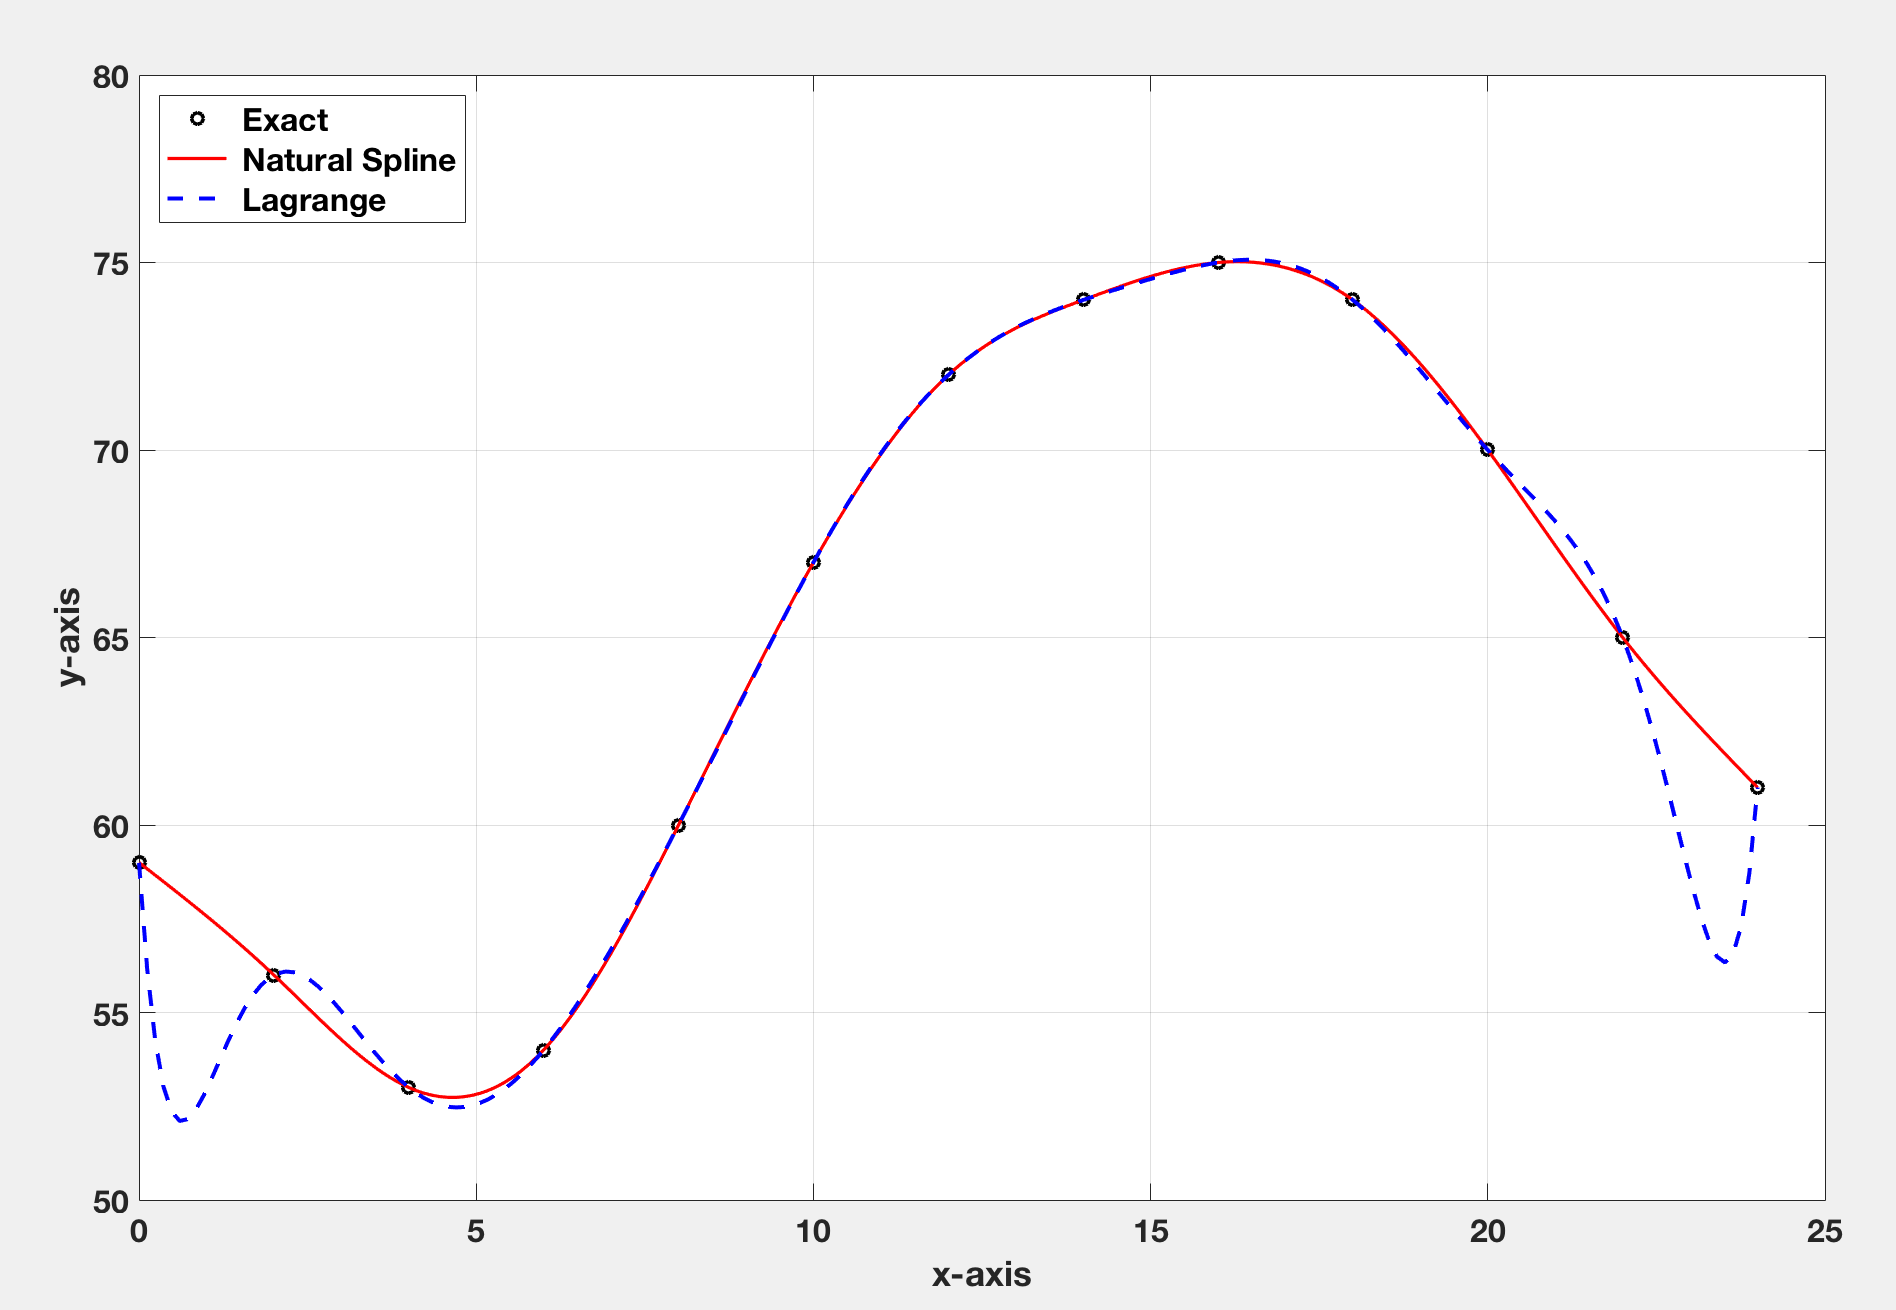
\includegraphics[width=\textwidth]{graph.png}
  \item \textit{What do each of the interpolation functions give us as the temperature at 11AM?}
    
    Lagrange interpolation gives 69.9 degrees.

    Natural spline gives 69.9 degrees.
  \item \textit{What do the two inperpolation functions predict the temperatue will be at 1AM the next day?}

    Lagrange interpolation gives 152 degrees.

    Natural spline gives 58.0 degrees.
  \item \textit{What do the two inperpolation functions predict the temperature will be at 9AM the next day? Explain the result of the spline interpolation.}

    Lagrange interpolation gives 452,300 degrees.

    Natural spline gives 0 degrees. This occurs due to the end conditions on natural spline, namely that $s_1''(x_1) = 0$ and $s_n''(x_{n+1}) = 0$. What happens past the endpoints of natural spline is restricted by this, and causes the function to tend to 0 as we look to extrapolate well beyond the end of the interpolation.
    
\end{enumerate}











\end{document}
